\section{The method}\label{sec:algo}
As presented in the previous section the eigenvalue problem of two electrons in a harmonic oscillator without any interaction terms can be easily solved. Looking at electrons in a quantum dot this calculation gains complexity. This is why we introduce the Variational Monte Carlo Method for estimating the electron states.
\subsection{Variational Monte Carlo method}
In the Variational principle, we take the eigenvalue problem from equation~\ref{glg:eigenvalue} and expand the wave function as following:
\begin{equation}
\varphi_0 = \sum_{\lambda=0}^{\infty} c_{0 \lambda} \psi_{\lambda},
\end{equation}
where $c_{0 \lambda}$ are coefficients.\\
In quantum mechanics the energy is the expectation value
\begin{align}
E = &\frac{\langle \psi_0 | \hat{H} | \psi_0 \rangle}{\langle \psi_0 | \psi_0 \rangle}\\
\intertext{So when we apply the expansion to this, we get:}
&\frac{\langle \varphi_0 | \hat{H} | \varphi_0 \rangle}{\langle \varphi_0 | \varphi_0 \rangle}\\
= &\frac{\sum_{\alpha,\beta}c_{0\alpha}^*c_{0 \beta} \int d\tau \psi_{\alpha}^*(\tau)\hat{H}\psi_{\beta}(\tau)}{\sum_{\alpha,\beta}c_{0\alpha}^*c_{0 \beta} \int d\tau \psi_{\alpha}^*(\tau)\psi_{\beta}(\tau)}\\
= &\frac{\sum_{\alpha} E_{\alpha} |c_{0\alpha}|^2}{\sum_{\alpha} |c_{0\alpha}|^2},
\end{align}
because by construction $\langle\psi_{\alpha}| \psi_{\beta}\rangle = \delta_{\alpha \beta}$ for eigenfunctions $\psi_{\alpha},\psi_{\beta}$.\\
We have to consider two cases now:
\begin{itemize}
\item If the expansion $\varphi_0$ is not the eigenfunction $\psi_0$ we get the an energy
\begin{equation}
E_0 \leqslant \frac{\langle \varphi_0 | \hat{H} | \varphi_0 \rangle}{\langle \varphi_0 | \varphi_0 \rangle}.
\end{equation}
\item If the expansion $\varphi_0$ corresponds exactly to the eigenfunction $\psi_0$ we get the exact energy
\begin{equation}
E_0 = \frac{\langle \varphi_0 | \hat{H} | \varphi_0 \rangle}{\langle \varphi_0 | \varphi_0 \rangle}.
\end{equation}
\end{itemize}
In the second case the variance of the energy
\begin{equation}
\mathrm{var}(E) = \langle H^2 \rangle - \langle H\rangle^2 = 0.
\end{equation}
As expansion wave function $\varphi_0$ we use a trial wave function we will call $\psi_T (\mathbf{r_1, r_2},\alpha, \beta)$, with $\alpha$ and $\beta$ being the variational parameters. In this report the trial wave function for two electrons has the form:
\begin{equation}
\psi_T(\mathbf{r_1,r_2}) = C \exp\left[-\alpha\frac{\omega}{2} (r_1^2+r_2^2)\right] \exp \left[ \frac{a_{12} r_{12}}{(1+\beta r_{12})} \right]
\end{equation}
with
\begin{align}
a_{12} =\left\{\begin{array}{cl} 1, & \mbox{for} \uparrow\downarrow\\ 1/3, & \mbox{for} \uparrow\uparrow,\downarrow\downarrow \end{array}\right]
\end{align}
and
\begin{equation}
r_{12} = \sqrt{\mathbf{r_1} - \mathbf{r_2}}.
\end{equation}
The factor $J = \exp \left[ \frac{a_{12} r_{12}}{(1+\beta r_{12})} \right]$ is called the Jastrow factor, which we will refer to later.\\
In order to find the wave function and its corresponding energy to the case we are considering, we compute the expectation value $E(\alpha, \beta)$ and find its minimum or alternatively the minimum of its variance $\mathrm{var}(E(\alpha, \beta))$. This procedure is used in section~\ref{sec:result}. For the six electron case, the variational wave function becomes as in equation~\ref{glg:6electron} and we can again search the minimum energy.\\
%Slater determinant -> six electron stuff
\subsection{Monte Carlo methods}
The basis of the method explained above are the Monte Carlo methods, which can be referred to as statistical simulation methods. The central building block of these methods is the propability distribution function (PDF), which is used to describe and characterize the physical problem. This does not restrict the method to statistical problems, but by displaying the desired solution in terms of PDF's, non-stochastic problems can be handled as well. During a Monte-Carlo simulation, random numbers must be generated covering an interval uniformly. Using these numbers, many random samples are taken from the PDF. In order to get the desired result the average of all samples is computed. According to this, the precision of the simulation rises with the amount of samples. The error has to be estimated to get an impression of the simulation's precision.\\
On the contrary of statistical random number-based methods, in standard mathematical modelling, the problem would be distretized and solved by a numerical approach.\\
\subsubsection{Pseudo-random number generation}\label{sec:ran}
As a main ingredient, random numbers play as important role in Monte-Carlo simulations and therefore have to be 'as random as possible'. The generation of truely random numbers is practically not possible, this is why the random numbers we work with are pseudo-random, generated by an algorithm fullfilling the criteria of
\begin{itemize}
\item generating equally distributed numbers in a given interval (usually [0,1])
\item repeating random number sequences seldom
\item being fast
\item generating insignificantly correlated numbers
\end{itemize}
I this report, we use random number generators explained in~\cite{numerical}, that are called \texttt{ran0} and \texttt{ran1}.\\
Furthermore, we generate random gaussian distributed random numbers using \texttt{gaussian}. 
% Jetzt nutzen wir andere 
\subsection{Metropolis algorithm}\label{sec:metropolis}
The difficult part of Monte-Carlo simulations is the selection rule for random states. One must find a method when to reject and when to accept the generated state. Precision and efficiency strongly depend on this rule. Supposing we have a distribution such as the one shown in figure~\ref{fig:distribution} and we have already picked an initial random variable at $r_i$. Since we are performing the simulation on many samples, we now have to pick a new random number keeping in mind, that there are two cases, which must be avoided:
\begin{itemize}
\item Choosing repeatedly numbers very close to the initial value such as $r_j$ in figure~\ref{fig:distribution}. We would then 'get stuck' around the interval of $r_i$ and therefore loose the overview of the function we are evalutating.
\item Jumping to numbers far away from the initial value, where the distribution is negligable, for example to $r_k$ in figure~\ref{fig:distribution}. 
\end{itemize}
\begin{figure}[htbp]
    \centering
    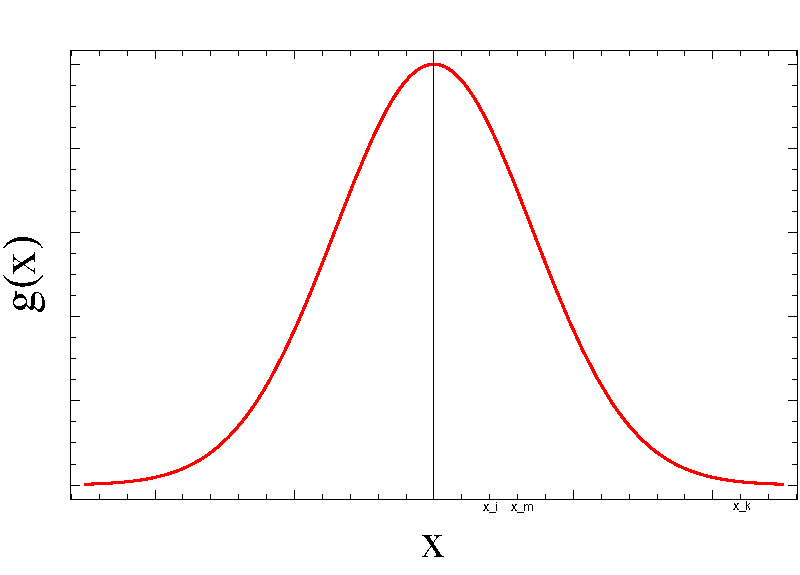
\includegraphics[scale=0.45]{distribution}
    \caption{Gaussian distribution showing problems in selection of random states}
    \label{fig:distribution}
\end{figure}
Preventing the simulation in creating biased averages and unprecise results is possible by using the Metropolis algorithm, which is a Markov process, satisfying both ergodicity and detailed balance.\\
Ergocidity in random processes means, that the time average of a sequence of events has to be the same as the average of all possible states, the so-called ensemble-average. In order to obey detailed balance, the process must follow a distribution, where the transition propability from state $i$ to state $j$ is the same as from state $j$ to state $i$ at equilibrium. This is also called reversibility.\\
Markov chains are referred to as random walks with selected propability to make a move, which is independent of the previous step. An example of this movement is the Brownian random walk shown in figure~\ref{fig:Brown}, where a particle moves in the $x$-$y$-plane with step length 1 preforming hundred steps. The propability of moving is the same for every direction. Using Markov processes, we can generate new random states and reach the most likely state (equilibrium) after a certain time.
%ergodicity
%detailed balance
\begin{figure}[htbp]
    \centering
    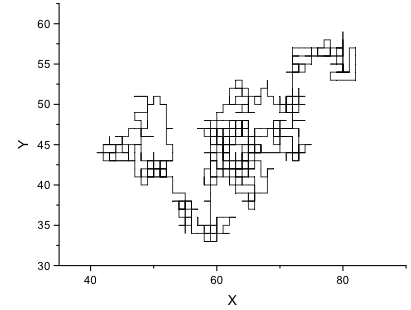
\includegraphics[scale=0.6]{Brown}
    \caption{Brownian random walk of 100 steps in $x$-$y$-plane and step length 1}
    \label{fig:Brown}
\end{figure}
\FloatBarrier
\subsubsection{Importance sampling}\label{sec:importance}
There are lots of examples in science, where biasing is disturbing and should be avoided. One example are the required unbiased uncorrelated random numbers in section~\ref{sec:ran}. In Monte-carlo methods, biasing can be a tool to increase the simulation's efficiency by preforming a Metropolis walk biased by the trial wave function. Since our problem is somewhat simular to a diffusion process in one dimension for one particle, we may use an approach based on the Fokker-Planck and the Langevin equation.\\
The 'old' and 'new' positions in space can be caluclated by
\begin{align}
r_{old} &= \eta\\
r_{new} &= r_{old} + \eta + \delta t D F_{old},
\end{align}
where $\eta$ denotes a gaussian distributed random variable, $\delta t$ refers to the time step, $D$ is the diffusion constant, which is in our case set to $D=0.5$ and $F_{old}$ is the quantum force at position $r_{old}$. Note, that $\eta$ are different random numbers.\\
The term responsible for biasing the walk in space $x$ is the quantum force, which leads the walk to regions with large trial wave function. In a brute force Metropolis algorithm, the propability of moving would be the same for all directions. The quantum force is
\begin{equation}
\mathbf{F} = 2 \frac{1}{\psi_T} \mathbf{\nabla} \psi_T
\end{equation}
In order to include this biasing in the Metropolis algorithm, we will replace
\begin{align}
q(r_{old},r_{new}) &= \frac{\vert \psi_T(r_{new})\vert^2}{\vert \psi_T(r_{old})\vert ^2}
\intertext{by}
q(r_{old},r_{new}) &= \frac{G(r_{old},r_{new},\delta t) \vert \psi_T(r_{new})\vert^2}{G(r_{new},r_{old},\delta t) \vert \psi_T(r_{old})\vert^2},
\intertext{where the quantity $G$ refers to the Greensfunction}
G(y,x,\delta t) &= \frac{1}{(4\pi D\delta t)^{3N/2}} \exp\left[-(y-x-D \delta t F(x))^2 \frac{1}{4D \delta t} \right].
\end{align}
\subsection{Analytical calculations}